The two component diagrams expose how the system architecture is build at two different level of abstraction: the High Level Component Diagram shows how the main subsystems are arranged and interconnected and what interfaces they use to communicate; the System Core Component Diagram, instead, contains a more detailed description of which software components have to be implemented to build the core of our system.\\
Under each diagram there are descriptions of the main functionalities performed by every component shown.

\begin{figure}[H]
\centering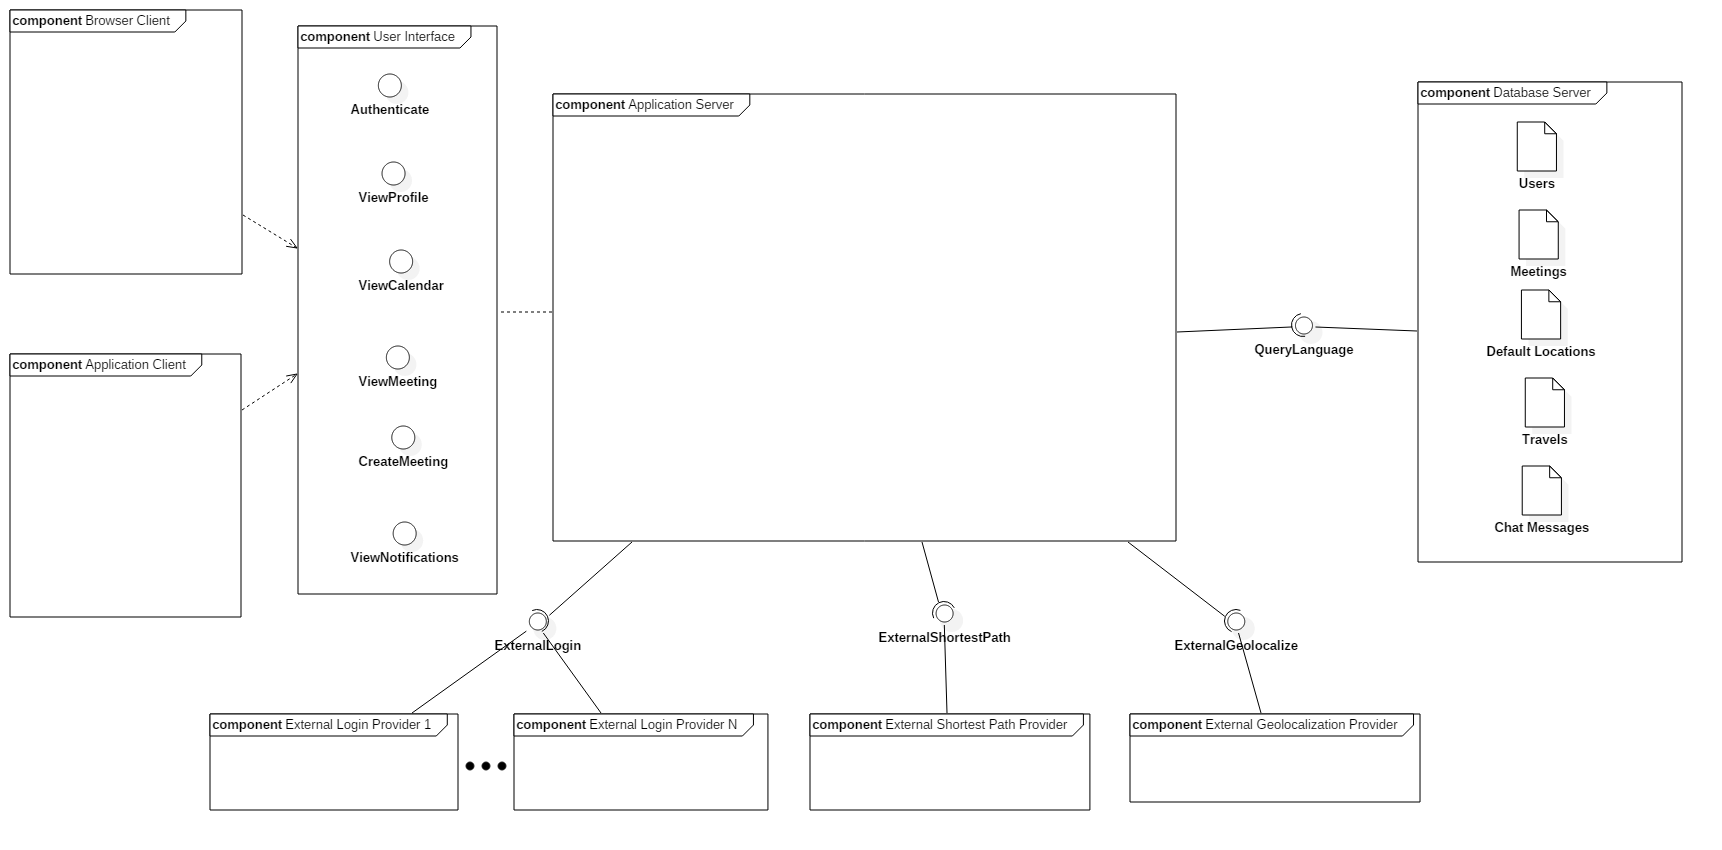
\includegraphics[width=\textwidth]{Images/UMLDiagrams/HighLevelComponentDiagram.png}
\caption{High Level Component Diagram}
\end{figure}

\begin{itemize}
\item \textbf{Route Manager}: manages the mapping between URLs and core system interfaces; it is the gateway for every request incoming from clients.
\item \textbf{Webpage Engine}: TO CHANGE!!! manages the building of web pages.
\item \textbf{Query Manager}: manages the interface towards the database, allowing the System Core to interact with it in a more abstract way.
\end{itemize}

\begin{figure}[H]
\centering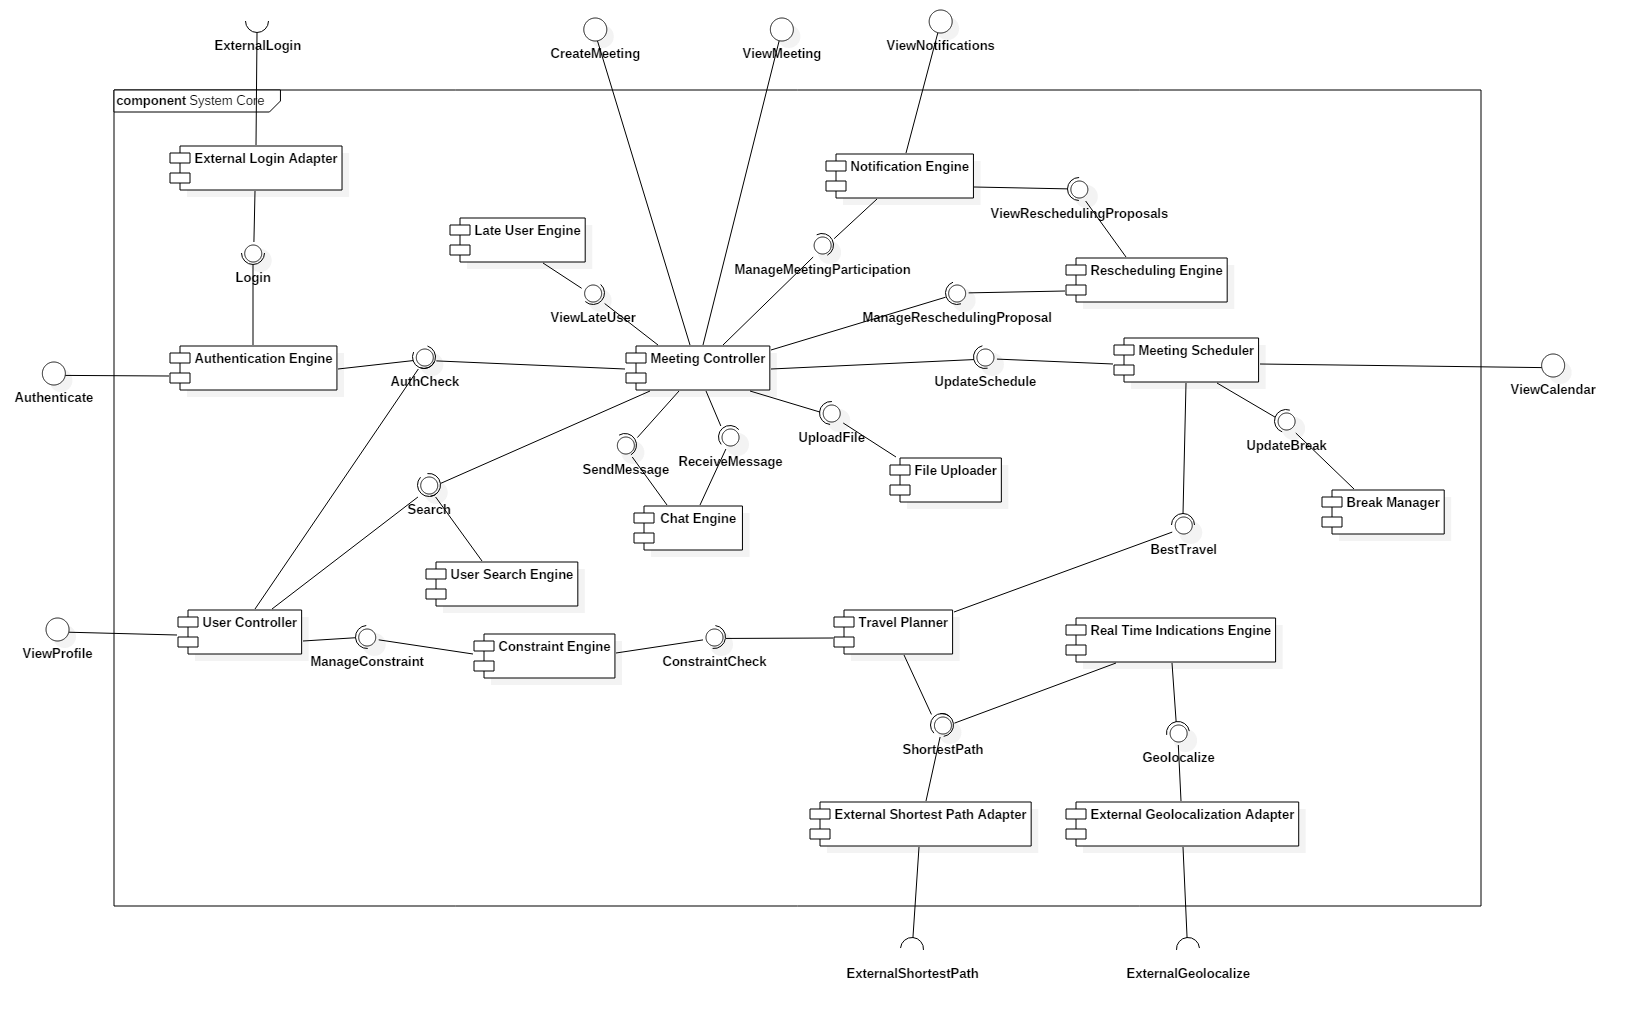
\includegraphics[width=\textwidth]{Images/UMLDiagrams/ApplicationComponentDiagram.png}
\caption{System Core Component Diagram}
\end{figure}

\begin{itemize}
\item \textbf{Authentication Engine}: manages everything related to registration and login and provides to the rest of the system an interface to check if a request comes from a user and, if so, from what user.
\item \textbf{External Login Adapter}: manages the interface towards external login providers.
\item \textbf{User Controller}: manages everything related to the users, such as their profile and their settings.
\item \textbf{User Search Engine}: manages the search of a user in the system by some keywords, such as their email or nickname.
\item \textbf{Constraint Engine}: manages all the constraints available in the system and provides an interface for the user to edit its own and an interface for checking if a specific constraint has to be enforced on a specific travel.
\item \textbf{Meeting Controller}: manages everything related to meetings, from users' and administrators' perspective.
\item \textbf{Chat Engine}: manages the chat system available in every meeting.
\item \textbf{Late User Engine}: uses the data about the positions of the users to extrapolate who's late for a meeting and create a dashboard for administrators to visualize it.
\item \textbf{File Uploader}: manages the upload of files for meetings.
\item \textbf{Travel Planner}: computes the best travel between two given locations for a given user.
\item \textbf{Real-Time Indications Engine}: manages the real-time indications given to a user to guide him to the next meeting.
\item \textbf{External Shortest Path Adapter}: manages the interface towards external shortest path providers.
\item \textbf{External Geolocalization Adapter}: manages the interface towards external geolocalization providers.
\item \textbf{Meeting Scheduler}: manages the users' schedules and the insertion of new meetings into it.
\item \textbf{Break Manager}: manages the flexible breaks updating their effective time whenever it's needed.
\item \textbf{Rescheduling Engine}: manages rescheduling proposals and their responses.
\item \textbf{Notification Engine}: manages all the notifications that are sent to users, such as warnings and meeting invitations.
\end{itemize}